\section{结果}

\subsection{信息渠道的双通道：书里哪些词被反复写}

先看最朴素的一层：全书逐字命中次数（表 II 括此图）。公开渠道一侧，东林 256、奏疏 202、弹劾 179、
上疏 88、诏狱 37、廷杖 35；隐秘渠道一侧，锦衣卫 207、东厂 122、特务 86、妖书 31、监视 24、
告发 11、谣言 10、党争 10、匿名 5、黑名单 5、流言 2。

\begin{figure}[!t]
\centering
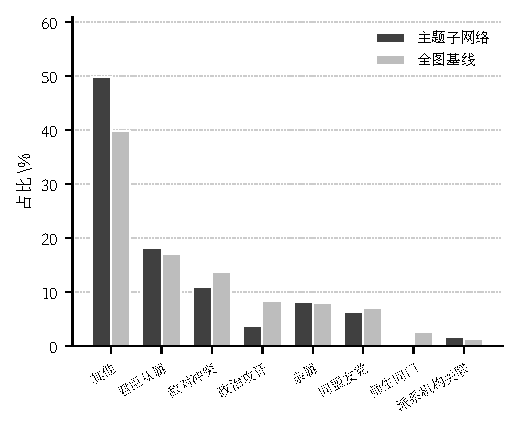
\includegraphics[width=\columnwidth,clip,trim=0 0 0 0]{fig_info_2.pdf}
\caption{信息机制的两种渠道在原书中的逐字命中次数。灰蓝为公开渠道（奏疏、弹劾、上疏、廷杖、诏狱、党争、
东林），棕橙为隐秘渠道（锦衣卫、东厂、西厂、特务、妖书、告密、告发、谣言、流言、黑名单、匿名、监视）。
所有词均经原书全文逐字核验，命中数 $\ge1$；「内厂」「厂卫」「揭帖」「榜文」「侦缉」「暗访」「风闻」「耳语」
命中为 0，已整体弃用不进图。}
\label{channels}
\end{figure}

Fig.\ref{channels} 里最重要的一件事不是两组谁高，而是**两组中间隔着一个数量级断层**：
公开渠道词集中在百次量级，隐秘渠道词从百次一路掉到个位数。以妖书案为例，原文写这份传单
「短短十几天内朝廷人人皆知」，传播速度本身就是被当作事件讲出来的；但对作者而言，
「告密」全书只出现 4 次。隐秘机制在书里是**事件**，不是**常设制度**——它一发生就被写成情节，
不发生时书中没有任何日常性描写。这一条是后文机构隐形结论的前置观察。

\subsection{攻讦占全关系的比重随时间上升，敌对冲突不升}

\begin{figure}[!t]
\centering
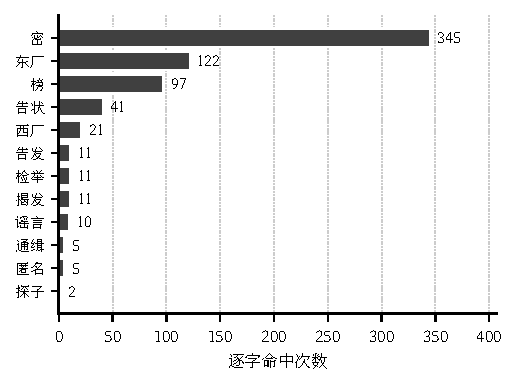
\includegraphics[width=\columnwidth,clip,trim=0 0 0 0]{fig_info_1.pdf}
\caption{政治攻讦与敌对冲突占该部全部关系的比重。柱为该部占比（左柱攻讦、右柱敌对），
折线连接同类的七部取值；横轴括号内标注该部攻讦关系数与该部关系总数。}
\label{bypart}
\end{figure}

Fig.\ref{bypart} 给出 $\pi_p(A)$ 与 $\pi_p(F)$。攻讦从第 1 部 5.6\% 走到第 6 部 19.9\%，
敌对冲突则在 13.1\%--30.8\% 之间无趋势地波动。取两端汇总：第 1--2 部合计 25/388 $=6.4\%$，
第 6--7 部合计 68/425 $=16.0\%$，比值 $2.48$；对照组敌对冲突同一口径 22.7\% 与 22.1\%，
比值 $0.98$。用一个不随时间变化的量做分母复核，比值 $2.48$ 不是分部规模差异造出来的。

\begin{table}[!t]
\centering
\caption{两组对照量的时间走向（分部口径）。}
\label{trend}
\small
\begin{tabular}{lrrrr}
\toprule
 & 第 1--2 部 & 第 6--7 部 & 比值 & 分母 \\\midrule
政治攻讦 & 6.4\% & 16.0\% & 2.48 & 388 / 425 \\
敌对冲突 & 22.7\% & 22.1\% & 0.98 & 388 / 425 \\
\bottomrule
\end{tabular}
\end{table}

旁证（章节年份中位数代理）：攻讦在 1368--1450 段占 11.8\%、1451--1550 段 39.4\%、
1551--1644 段 48.8\%，同样单调上升；敌对冲突为 24.9\% / 23.5\% / 51.6\%，后段同样抬升但前两段持平。
两路口径同号，主结论以分部口径为准。

\subsection{攻讦是跨阵营的，而且越来越跨阵营}

用完整派系串判定两端是否同阵营：193 条攻讦里有 86.0\% 是跨阵营、14.0\% 同阵营。
逐部看，第 5 部跨阵营 96.0\%、第 6 部 97.4\%、第 7 部 70.0\%、第 1 部 72.7\%：
跨阵营比例在中段最高，末段回落。这里要说明一个口径反差：若把派系折叠到根类
（「明朝·阉党」与「明朝·文官」都算「明朝」），同阵营会虚高到 76.7\%——因为 1231 人中
有 171 人只挂了「明朝」这一个根类。完整串口径给出的 86.0\% 才是可用值，
正文不报折叠口径的数字。

攻讦端点分布相当分散：193 条关系涉及 202 个不同人物，基尼系数 0.3798，Top-10 端点只占全部端点次数的
21.0\%。端点名册的前几名是张居正 11 次、申时行 11 次、魏忠贤 9 次、刘瑾 8 次、王守仁 8 次、
朱翊钧 8 次。攻讦与敌对的端点集只有 86 人重合，Jaccard 系数 0.219——
**两者盯的不是同一批人**，这排除了「攻讦只是敌对换个标签」的读法。

\begin{table}[!t]
\centering
\caption{攻讦关系端点前 8 名及其图谱位置。}
\label{topend}
\small
\begin{tabular}{lcrrr}
\toprule
人物 & 攻讦次数 & 度数 & 出场章 & 派系 \\\midrule
张居正 & 11 & 66 & 23 & 明朝·万历朝 \\
申时行 & 11 & 32 & 9 & 明朝·内阁（后首辅）\\
魏忠贤 & 9 & 67 & 12 & 明朝·阉党 \\
刘瑾 & 8 & 34 & 8 & 明朝 \\
王守仁 & 8 & 50 & 12 & 明朝·文官 \\
朱翊钧 & 8 & 52 & 30 & 明朝·万历朝 \\
严嵩 & 7 & 59 & 17 & 明朝·嘉靖朝·文官 \\
高拱 & 7 & 59 & 12 & 翰林院 \\
\bottomrule
\end{tabular}
\end{table}

\subsection{机构隐形，代理人在场}

\begin{figure}[!t]
\centering
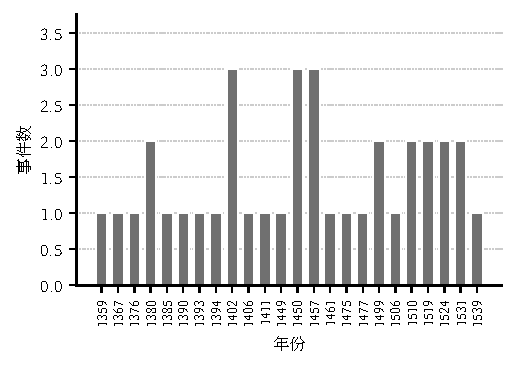
\includegraphics[width=\columnwidth,clip,trim=0 0 0 0]{fig_info_3.pdf}
\caption{信息型机构与其代理人的结构位置。三组分柱依次为平均关系度数、平均出场章节数、占攻讦关系端点的比重。
厂卫系按角色／派系中是否出现锦衣卫、东厂、西厂、内行厂辨认；内廷宦官按是否出现太监、宦官辨认；
两者有交集但不合并计数。}
\label{inst}
\end{figure}

Fig.\ref{inst} 与表 IV 给出本文最反直觉的一组数字。厂卫系 29 人平均度数 3.76，全库 3.78，
比值 $0.99$；平均出场章节 2.07 对全库 2.22，比值 $0.93$；作为攻讦端点的次数只占 3.6\%。
也就是说：**写了 207 次「锦衣卫」的这套机构，在 1231 人的关系网络里和一条平均线没有区别。**
对照内廷宦官 51 人：平均度数 6.10（$1.61$ 倍）、平均章节 2.57（$1.16$ 倍）、占攻讦端点 10.1\%。

\begin{table}[!t]
\centering
\caption{厂卫系、内廷宦官与全库基线的结构位置。}
\label{instable}
\small
\begin{tabular}{lrrrcc}
\toprule
 & 人数 & 平均度数 & 平均章节 & 攻讦端点占比 & 度数比值 \\\midrule
厂卫系 & 29 & 3.76 & 2.07 & 3.6\% & 0.99 \\
内廷宦官 & 51 & 6.10 & 2.57 & 10.1\% & 1.61 \\
全库基线 & 1231 & 3.78 & 2.22 & --- & 1.00 \\\bottomrule
\end{tabular}
\end{table}

两条佐证书内事实，供读者核对话语与结构的错位。其一，「卢忠是锦衣卫」，随即写他「勾结同事锦衣卫李善，
去向朱祁钰告密，罪名是阴谋复辟」——执行者是具体的人，被执行的机构只作身份标记；
另一处「王世贞被列入了严嵩的黑名单」，杀伤来自名单而非审判。
机构在书里是**标签**，在图谱里是**空节点**；真正成为节点、并且被反复拉进攻讦关系的是它背后的人
（魏忠贤、刘瑾、冯保、尚铭一类）。这不是数据有错，而是抽取口径天然偏向有名字的个人。

\subsection{攻讦的章节归属率远高于全库}

一个容易被漏掉的口径事实：939 条关系（40.4\%）标为「推导」、没有章节出处，
但攻讦类 193 条里只有 1 条是推导，章节归属率 99.5\%。全库归属率 59.6\%。
这说明攻讦边几乎全部来自逐章的人工标注，不是自动共现补出来的。
对本文是好消息（攻讦数据比平均更可靠），对本文也是坏消息（**抽取的覆盖面本身是不均匀的**，
这构成限制节的一条）。
